\begin{figure}[H]
\centering
\resizebox{0.3\textwidth}{!}{
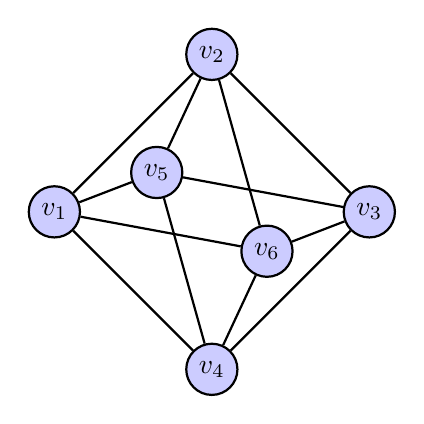
\begin{tikzpicture}[
  scale=1.0,
  vnode/.style={circle, draw=black, fill=blue!20, thick, inner sep=0pt, minimum size=6.5mm},
  edge/.style={thick, draw=black}
]
  % Vértices exteriores (cuadrado C4)
  \node[vnode] (v1) at (-2, 0) {$v_1$};
  \node[vnode] (v2) at (0, 2) {$v_2$};
  \node[vnode] (v3) at (2, 0) {$v_3$};
  \node[vnode] (v4) at (0, -2) {$v_4$};

  % Vértices polo interior/exterior (conectados a todo el C4)
  \node[vnode] (v5) at (-0.7, 0.5) {$v_5$};
  \node[vnode] (v6) at (0.7, -0.5) {$v_6$};

  % Aristas del cuadrado exterior
  \draw[edge] (v1) -- (v2) -- (v3) -- (v4) -- (v1);

  % Conexiones del vértice v5 (polo superior/interior)
  \draw[edge] (v5) -- (v1);
  \draw[edge] (v5) -- (v2);
  \draw[edge] (v5) -- (v3);
  \draw[edge] (v5) -- (v4);

  % Conexiones del vértice v6 (polo inferior/interior)
  \draw[edge] (v6) -- (v1);
  \draw[edge] (v6) -- (v2);
  \draw[edge] (v6) -- (v3);
  \draw[edge] (v6) -- (v4);

\end{tikzpicture}}%
\caption{Un grafo simple}
\end{figure}
